% This file was created by matlab2tikz.
%
%The latest updates can be retrieved from
%  http://www.mathworks.com/matlabcentral/fileexchange/22022-matlab2tikz-matlab2tikz
%where you can also make suggestions and rate matlab2tikz.
%
\documentclass[tikz]{standalone}
\usepackage[tuenc]{fontspec}
\setmainfont{FreeSerif}
\usepackage{pgfplots}
\usepackage{grffile}
\pgfplotsset{compat=newest}
\usetikzlibrary{plotmarks}
\usetikzlibrary{arrows.meta}
\usepgfplotslibrary{patchplots}
\usepackage{amsmath}
\usepackage{pgfplots}
\usepackage{tikz}
\usetikzlibrary{matrix,chains,positioning,decorations.pathreplacing,arrows}

\begin{document}
\definecolor{mycolor1}{rgb}{0.00000,0.44700,0.74100}%
\scriptsize
% Listing 2: Tex for neural network pipeline
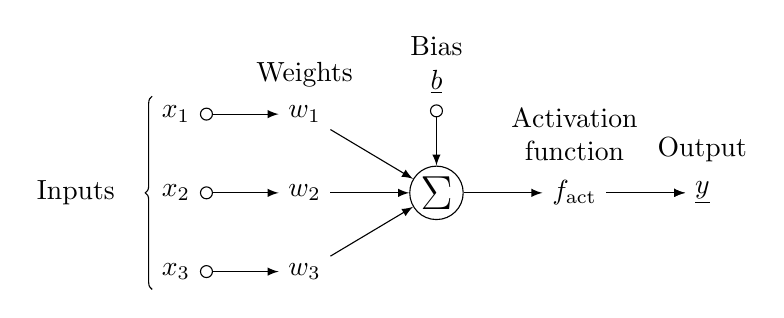
\begin{tikzpicture}[
% define styles
init/.style={
	draw,
	circle,
	inner sep=1pt,
	font=\LARGE,
	join = by -latex
},
squa/.style={
	font=\normalsize,
	join = by -latex
}
]
% Top chain x1 to w1
\begin{scope}[start chain=1]
\node[on chain=1] at (0,1cm)  (x1) {$x_1$};
\node[on chain=1,label=above:Weights,join=by o-latex] (w1) {$w_1$};
\end{scope}
% Middle chain x2 to output
\begin{scope}[start chain=2]
\node[on chain=2] (x2) {$x_2$};
\node[on chain=2,join=by o-latex] {$w_2$};
\node[on chain=2,init] (sigma) {$\displaystyle\Sigma$};
\node[on chain=2,squa,label=above:{\parbox{2cm}{\centering Activation\\ function}}]   {$f_{\rm act}$};
\node[on chain=2,squa,label=above:Output,join=by -latex] {$\underline{y}$};
\end{scope}
% Bottom chain x3 to w3
\begin{scope}[start chain=3]
\node[on chain=3] at (0,-1cm)
(x3) {$x_3$};
\node[on chain=3,join=by o-latex]
(w3) {$w_3$};
\end{scope}
% Bias
\node[label=above:\parbox{2cm}{\centering Bias \\ $\underline{b}$}] at (sigma|-w1) (b) {};
% Arrows joining w1, w3 and b to sigma
\draw[-latex] (w1) -- (sigma);
\draw[-latex] (w3) -- (sigma);
\draw[o-latex] (b.north) -- (sigma);
% left hand side brace
\draw[decorate,decoration={brace,mirror}] (x1.north west) -- node[left=10pt] {Inputs} (x3.south west);

\end{tikzpicture}

\end{document}
